\documentclass[11pt,a4paper]{article}
\usepackage[T1]{fontenc}
\usepackage[utf8]{inputenc}
\usepackage{lmodern}
\usepackage[margin=2.5cm]{geometry}
\usepackage{amsmath,amssymb}
\usepackage{booktabs}
\usepackage{graphicx}
\usepackage[hidelinks]{hyperref}
\hypersetup{pdfauthor={Gianni Pilotti},pdftitle={One-Day Value at Risk for a Multi-Asset EUR Portfolio},pdfcreator={},pdfproducer={}}
\setlength{\parindent}{0pt}
\setlength{\parskip}{6pt}

\title{One-Day Value at Risk for a Multi-Asset EUR Portfolio}
\author{Gianni Pilotti}
\date{}

\begin{document}
\maketitle

\section{The Core Idea}
Value at Risk (VaR) answers one question: how much can the portfolio lose in one day, with 99\% confidence? Expected shortfall (ES) adds a second: if the loss does exceed the VaR, how large is it on average?

The repository applies four VaR models to one portfolio and tests them out of sample. The portfolio is held by a EUR investor: four Paris stocks, three US stocks, a US Treasury ETF (TLT) and Ethereum, rebalanced daily to fixed weights.

\begin{itemize}
\item \textbf{Why compare models:} the choice of distribution moves the 99\% VaR by about 0.4 percentage points and the ES by more than 1 point.
\item \textbf{Why backtest:} a model that fits the full sample can still fail day by day.
\end{itemize}

\section{Method}
\subsection{Data and portfolio}
Yahoo Finance adjusted closes, 2020 to 2025. USD assets are converted to EUR with EURUSD, so FX risk is part of the result. Only days where every asset has a close are kept, which gives 1,494 daily simple returns. Simple returns are used because they aggregate across assets with the weights; log returns do not.

Weights: 10\% each in LVMH, Sanofi, L'Or\'eal, Airbus, Apple, Microsoft, NVIDIA and Ethereum, and 20\% in TLT. With $r_t=\sum_i w_i r_{i,t}$, the full-sample portfolio has an annualised volatility of 20.2\%, skew of $-0.42$ and excess kurtosis of 6.8.

VaR and ES are reported as positive losses with a zero mean. With confidence $\alpha=0.99$:

\subsection{Historical}
\[
\mathrm{VaR}=-q_{1-\alpha}(r),\qquad
\mathrm{ES}=-\mathbb{E}\left[r \mid r\le q_{1-\alpha}\right],
\]
where $q_{1-\alpha}$ is the empirical 1\% quantile.

\subsection{Normal}
With $z=\Phi^{-1}(\alpha)$ and $\sigma$ the sample standard deviation:
\[
\mathrm{VaR}=z\,\sigma,\qquad
\mathrm{ES}=\sigma\,\frac{\varphi(z)}{1-\alpha}.
\]

\subsection{Student-t}
The t distribution is fitted by maximum likelihood with a zero location, giving $\nu$ and a scale $s$. With $q=t_\nu^{-1}(\alpha)$:
\[
\mathrm{VaR}=s\,q,\qquad
\mathrm{ES}=s\,\frac{f_\nu(q)}{1-\alpha}\cdot\frac{\nu+q^2}{\nu-1}.
\]

\subsection{Monte Carlo (Student-t scenarios)}
Draw 100,000 joint scenarios for the nine assets: $x = z\,\sqrt{(\nu-2)/\nu}\,/\sqrt{\chi^2_\nu/\nu}$, where $z=L\varepsilon$, $L$ is the Cholesky factor of the sample covariance and $\varepsilon\sim N(0,I)$. The scaling keeps the sample covariance while adding fat tails. The degrees of freedom $\nu$ come from the portfolio fit above. The portfolio loss is $-w^\top x$, and VaR and ES are read with the historical estimator on the simulated losses (seed 42).

\subsection{Backtest}
Each day, VaR is estimated on the previous 250 days only and compared with the next day's return. A breach is a loss larger than the VaR. A fifth model, EWMA, is added: a normal VaR with $\sigma^2=\sum_k \lambda^k r_{t-k}^2 \big/ \sum_k \lambda^k$ and $\lambda=0.94$.

\begin{center}
\begin{tabular}{@{}lp{4.6cm}p{6.2cm}@{}}
\toprule
Test & Question & Statistic \\
\midrule
Kupiec & Is the breach count consistent with 1\%? & $LR=-2\ln\dfrac{(1-p)^{n-x}p^x}{(1-\hat p)^{n-x}\hat p^x}$, $\hat p=x/n$ \\
Christoffersen & Are breaches independent? & Markov chain of breaches against a constant rate \\
\bottomrule
\end{tabular}
\end{center}
Both statistics are compared with a $\chi^2_1$ distribution. Here $n$ is the number of days, $x$ the number of breaches and $p=1\%$.

\section{Results}
\textbf{Full sample} (1,494 days, one-day 99\%, in \% of portfolio value):

\begin{center}
\begin{tabular}{@{}lcc@{}}
\toprule
Model & VaR 99\% & ES 99\% \\
\midrule
Historical & 3.37 & 4.77 \\
Normal & 2.97 & 3.40 \\
Student-t & 3.37 & 4.63 \\
Monte Carlo (Student-t) & 3.40 & 4.65 \\
\bottomrule
\end{tabular}
\end{center}

The normal model gives a lower VaR and ES than the historical one, so it misses the tails. The five worst days are all in 2020 except 13 June 2022 ($-5.45\%$); the worst, 12 March 2020, is $-11.06\%$. Without 2020, the historical ES falls from 4.77\% to 3.70\%.

\textbf{Out-of-sample backtest} (1,244 days, 4 January 2021 to 31 December 2025, 12.4 breaches expected):

\begin{center}
\begin{tabular}{@{}lcccc@{}}
\toprule
Model & Breaches & Rate (\%) & Kupiec $p$ & Christoffersen $p$ \\
\midrule
Historical & 19 & 1.53 & 0.083 & 0.032 \\
Normal & 20 & 1.61 & 0.048 & 0.039 \\
EWMA & 21 & 1.69 & 0.026 & 0.048 \\
Student-t & 12 & 0.96 & 0.900 & 0.004 \\
\bottomrule
\end{tabular}
\end{center}

\begin{itemize}
\item \textbf{Count:} the Student-t model matches the expected number of breaches. Normal and EWMA fail the Kupiec test at 5\%.
\item \textbf{Clustering:} all four models fail the Christoffersen test. The Student-t model has the right count but the clustering is worst.
\item \textbf{Risk source:} Ethereum is 10\% of capital and 28.3\% of portfolio volatility. NVIDIA adds 18.5\%. TLT is 20\% of capital and 3.2\%.
\end{itemize}

\begin{figure}[h]
\centering
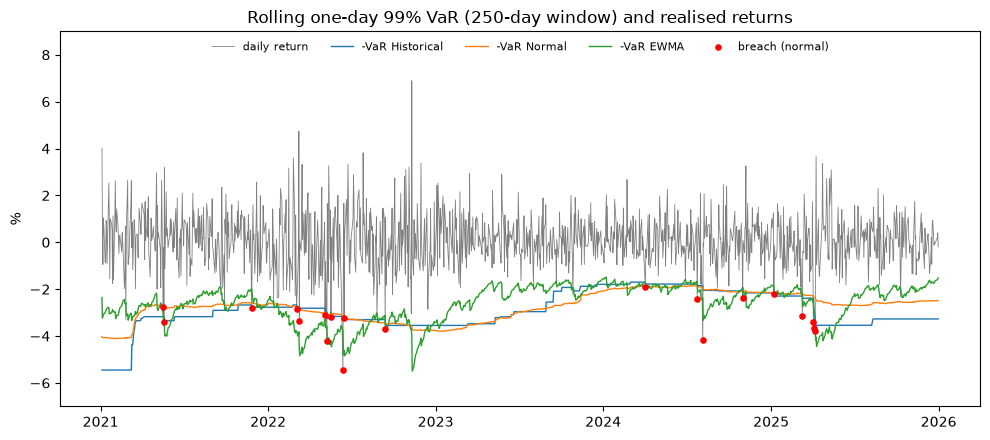
\includegraphics[width=0.95\textwidth]{../figures/rolling_var_backtest.png}
\caption{Rolling one-day 99\% VaR (250-day window) and realised returns. Red dots are normal-model breaches.}
\end{figure}

\section{Worked Example}
\textbf{Normal VaR and ES} with an illustrative daily volatility of $\sigma=1.27\%$ (close to $20.2\%/\sqrt{252}$):
\begin{align*}
z &= \Phi^{-1}(0.99) = 2.3263,\qquad \varphi(z)=0.02665,\\
\mathrm{VaR} &= 2.3263\times 1.27\% = 2.95\%,\\
\mathrm{ES} &= 1.27\%\times\frac{0.02665}{0.01} = 1.27\%\times 2.665 = 3.38\%.
\end{align*}
The notebook gives 2.97\% and 3.40\% because it uses the unrounded volatility. On an illustrative EUR 1,000,000 portfolio, the historical VaR of 3.37\% is EUR 33,700.

\textbf{Kupiec test} for the Student-t model: $n=1244$, $x=12$, $p=0.01$, so the expected count is $12.44$.
\begin{align*}
\hat p &= 12/1244 = 0.00965,\\
LR &= 0.0159 \quad\Rightarrow\quad p\text{-value}=0.900.
\end{align*}
For the normal model, $x=20$ gives $LR=3.919$ and a $p$-value of $0.048$, below 5\%.

\section{Limits}
\begin{itemize}
\item \textbf{Short sample:} 2020 contains the March crash, which drives the historical ES. The sample is six years, so the 1\% tail rests on about 15 observations.
\item \textbf{Fixed weights:} daily rebalancing to fixed weights is assumed, with no transaction costs, and the portfolio is not a real book.
\item \textbf{One-day horizon:} the zero-mean assumption is standard at one day but does not hold for longer horizons.
\item \textbf{Weekend moves:} Ethereum trades every day, so its weekend moves are folded into the Monday return.
\item \textbf{Test power:} with about 12 expected breaches, Kupiec and Christoffersen have limited power. The results are model outputs, not recommendations.
\end{itemize}

\end{document}
